\documentclass{article}
\usepackage[utf8]{inputenc}
\usepackage[T1]{fontenc}
\usepackage[french]{babel}
\usepackage{graphicx}
\usepackage{subcaption}
\usepackage{wrapfig}
\usepackage{color}
\usepackage{float}
\usepackage{colortbl}
\usepackage{multirow}
\usepackage{amsmath}
\usepackage{diagbox}
\usepackage{amssymb}
\usepackage{mathrsfs}
\usepackage{hyperref}
\usepackage{pgfplots}
\hypersetup{colorlinks=true, linkcolor=black, bookmarksopen=true,pdffitwindow=true,pdfauthor={Pierrick Rauby}, pdftoolbar=false}
\usepackage[top=2cm, bottom=2cm, left=3cm, right=3cm]{geometry}
\title{Comment enrichir son Double Diplôme à GeorgiaTech?}
\date{Mise à jour, Spring, 2020}

\author{
  Eymard, Prevost\\
  \texttt{Li215}
  \and
  Pierrick, Rauby\\
  \texttt{Me214}
  \and 
  Sébastien, Séqueira\\
  \texttt{Bo216}
}

\begin{document}{}
\maketitle 

\section{Introduction}
Vous trouvez que 6 mois aux US c'est un peu court ? Vous aimeriez travailler dans ce pays ? Vous souhaitez prolongez quelque peu vos études pour affiner votre projet professionnel ? Le doctorat vous intéresse mais vous n'êtes pas encore sûr ? Ou êtes vous tout simplement curieux et êtes à la recherche d'une expérience nouvelle et facilement valorisable ? Ce document est pour vous !

L'objectif est ici de présenter certains conseils qui vous permettront de diminuer les frais de vos études de manière potentiellement très conséquente, d'allonger la durée de vos études, et de gagner en expérience. 
Sont présentés ici deux parcours:
\begin{itemize}
\item le GRA (Graduate Research Assistantship)
\item le GTA (Graduate Teaching Assistant)
\end{itemize}
Un petit détail avant d'entrer dans le dur du sujet: certains n'ont probablement pas envie de prolonger leurs études et souhaiteraient commencer à travailler aux US dès la fin de leur premier semestre. Sachez que ce sera très compliqué. Pas impossible, mais vraiment pas évident, car vous n'avez pas de visa de travail et les entreprises rechignent souvent à sponsoriser (sauf quelques exceptions). Par contre sachez que si vous arrivez à rester en tant qu'étudiant à GT un semestre de plus, vous aurez accès à un OPT (optional practical training) qui vous permettra de travailler aux US pendant 3 ans. Tous vos rêves seront désormais possibles (en tout cas plus probables) !

\section{Description des différentes options}
\subsection{Le GRA (Graduate Research Assistanship)}


 Le GRA (Graduate Research Assistanship) consiste à travailler pour un professeur de GT en échange (pas toujours mais souvent) d'un salaire (jusqu'à 
\$ 2350 / mois).Souvent, le laboratoire  pour lequel les étudiants travaillent finance aussi les frais de scolarité  (voir section \ref{Etre paye} pour plus de détails). Le travail peut être théorique ou appliqué, en fonction du professeur, cela vous demandera certainement la majeur partie de votre temps en semaine. Il est généralement d'une durée de 2 semestre, les professeurs ne sont pas intéressés pour un seul semestre.

Comme exemples de travail, il y a: 
\begin{enumerate}
\item travail sur un projet de maintenance prédictive pour une entreprise industrielle dans le cadre de la détection de défauts sur des roulements à billes (beaucoup de programmation en python et d'analyse de donnée dans le cloud).
\item étude sur l'utilisation des batteries de voitures électriques comme source d'énergie pour le domicile, et les économies réalisées.
\item optimisation thermique des moteurs électriques pour l'industrie automobile, très accès logiciel de simulation.
\end{enumerate}

A noter que le GRA est très souvent couplé à un Master Thesis dans le cas d'un étudiant étranger. En effet, le GRA seul rapporte un salaire, mais ne compte pas en terme de crédits académiques, au contraire du GRA avec une Master Thesis.

\subsection{Master Thesis}

La Master Thesis permet généralement de faire valoir votre travail de GRA d'un point de vue académique. Lorsque vous arrivez à Atlanta il vous reste 12 crédits académiques à valider pour obtenir votre diplôme et pour cela vous avez plusieurs choix:
\begin{itemize}
\item prendre 4 cours (1 cours = 3 crédits académique).
\item prendre 1 cours et une Master Thesis (9 crédit académiques) d'une durée minimum de deux semestres. 
\end{itemize}

Par ailleurs, pour conserver son statut de VISA F1, la loi américaine impose que chaque étudiant étranger ait au minimum 12 crédits hours. Attention: différents de crédit académiques, ils représentent votre charge de travail du semestre.

Donc si vous avez un GRA sans Thesis, vous devez prendre 4 cours pour avoir vos 12 crédits hours du semestre et conserver votre VISA F1, c'est la galère assurée. La technique est donc de faire une Master Thesis qui vous permet de prendre moins de cours car vous pouvez décider d'attribuer autant de credit hours (jusqu'à 21) que vous voulez à ce travail, par contre, elle comptera toujours pour 9 crédits académiques. 

La Master Thesis développe une problématique de recherche en lien avec votre GRA. Vous allez travailler dans une équipe de recherche sur des problématiques théoriques ou expérimentales et rédiger une thèse sur le sujet de votre choix, en général en lien avec votre GRA. En fonction du lab et du professeur qui vous encadre vous serez plus ou moins guidés et même si un problématique initiale sera définie, vous ne saurez pas, a priori, si l'approche que vous étudiez mènera à des résultats concluants. 

Ceci amène un deuxième point : la master Thesis est un travail de recherche plutôt solitaire et le travail d'équipe n'est donc pas aussi omniprésent qu'en entreprise. Par ailleurs, ceci vous oblige à développer une vraie autodiscipline ce qui est très formateur pour de futurs projets. Mais cette autonomie vous permet d'aménager facilement votre emploi du temps : le lieu de travail, la quantité de travail sont assez flexibles généralement puisque ce qui compte c'est l'objectif final du projet. 
Il vous apprendra à lire des papiers scientifiques et en extraire des informations (pour ça très bon cours d'un mois proposé chaque semestre par Georgia Tech sans engagement de notes: ECE-ME SW donné par Dr. Lauren Lukkarila). 

De plus, contrairement à un diplôme de PhD, juste le fait d'avoir un Master avec Thesis ne va pas vraiment vous distinguer d'une personne avec un Master sans Thesis, d'un point de vue qualification. Cependant, tout ce que vous aurez appris en un an et le travail que vous aurez produit vous donnera bien plus d'arguments si vous cherchez un travail dans le même domaine que celui de votre recherche.
\subsection{GTA (Graduate Teaching Assistant)}
Plutôt que de vous tourner vers de la recherche avec un GRA vous pouvez vous tourner vers des tâches d'enseignements et devenir Teaching Assistant (TA) pour un cours,  attention, une bonne maîtrise de la langue et de la pédagogie sont pré-requis pour cette position. Généralement il s'agit d'un cours de niveau undergraduate d'une matière que vous maitrisez, les mathématiques par exemple sont un gros point fort des élèves de classes préparatoires par rapport aux américains. Vous pouvez aussi enseigner des matières de niveau graduate, pour cela il faudra en général avoir déjà pris le cours et avoir obtenu un A. 

Les tâches que vous serez amenés à effectuer dans le cadre d'un GTA sont diverses et dépendent à la fois du professeur et du cours: préparer les sujets, correction de devoirs maison et des examens, remplacer le professeur quand il est en conférence, tenir les offices hours. 

Enfin, rien ne vous empêche de cumuler à la fois la position de GRA et celle de GTA, mais cela est très chronophage.

Par la suite sont présentés les avantages et autres détails concernant ces parcours. A noter que nous mettrons un fort accent sur la master thesis couplée à un GRA. C'est de loin l'option la plus choisie puisqu'elle présente de très nombreux avantages (à moins que vous vouliez impérativement commencer à travailler janvier prochain). 


\section{Avantages}
\subsection{Être payé \label{Etre paye}}
\subsubsection{Les différents statuts et leurs conséquences financières }Tout travail effectué dans le cadre des parcours présentés ci-dessus ouvrent le droit à des compensations financières à l'exception du master thesis qui fait seul qui n'est pas rémunéré. Ces compensations sont de deux types:
\begin{itemize}
\item un tuition waiver (réduction des frais de scolarité) de \$15 000/ semestre à moins de \$2000/semestre.
\item un salaire, en général de \$2350 brut, mais certains lab ne paient pas autant. 
\end{itemize}

Pour les GRA et GTA, vous n'aurez pas forcément un tuition waiver, assurez vous de bien confirmer avec le professeur. 

En fonction du moment où vous rejoignez les parcours dans le semestre vous pouvez ne pas avoir droit au tuition waiver et donc n'avoir le droit qu'à un salaire (voir explications ci-après). 


\begin{table}[h]
\begin{center}
\begin{tabular}{|c|c|c|c|}
\hline
 &  GRA &  GTA  & GA \\
% & (Graduate Research Assistant) & (Graduate Teaching Assistant) & (Graduate Assistant)\\
\hline
Frais de scolarité & tuition waiver & tuition waiver & pas de réduction  \\
& $\rightarrow$ réduit de \$15 0000 & $\rightarrow$ réduit de \$15 0000 & $\rightarrow$ \$15 000/semestre \\
&à \$2000/semestre&à \$2000/semestre&\\
\hline Salaire brut & jusqu'à  \$2350/mois & jusqu'à  \$2350/mois & jusqu'à \$2350/mois \\
\hline
\end{tabular}
\end{center}
\caption{Salaires et reduction de frais de scolarité par position}
\label{Salaires et reduction de frais de scolarité par position}
\end{table}


\subsubsection{Tu trouves un laboratoire, que se passe-t-il ensuite ?}
C'est la question que tu dois avoir maintenant. On va prendre un exemple: tu es en stage SFE en Spring après ton semestre de Fall GTL, et tu te prépares à partir pour ton semestre de Fall à GeorgiaTech Atlanta. Trois cas se présentent: 
\begin{enumerate}
\item Tu trouves un post de GRA ou de GTA avant le début du semestre, tu peux alors appliquer le tuition waiver et payer des frais de scolarité fortement réduits. Dans le cadre d'un GRA couplé avec une master thesis, il faut aussi suivre les procédures de changement de statut (de Master sans Thesis à Master avec Thesis) avant la deadline de fin de Registration pour les cours. Ce changement de statut implique une extension de ton I-20 (sans changer de VISA), pour la durée de Thesis. Par ailleurs, et afin de refléter la charge de travaille liée au master Thesis, il faudra ajouter le cours Master Thesis 7000, et assigner 9 crédits hours manuellement à ce cours et tu indiquant ton professeur référent qu'ils appellent Advisor pour ta recherche.
\item Tu trouves ton lab après la deadline. Dans ce cas tu peux toujours te mettre d'accord avec ton futur advisor pour avoir le statut de GRA le semestre suivant. Il faudra alors faire des démarches avec l'administration de GeorgiaTech Atlanta afin d'étendre l'I-20 pour la durée du master Thesis. 
Note : tu as jusqu'à la première semaine de décembre pour trouver un GRA / Master Thesis pour le Spring de l'année suivante.
\item Enfin, il arrive que certains professeurs n'arrivent pas à remplir leur équipe de GRA ou de GTA, ils pourront alors t'embaucher en tant que GA après la deadline de registration mais dans ce cas, rappelons que tu ne pourras plus profiter d'un tuition waiver. 
 \end{enumerate}

\paragraph{Remarque: }si tu trouves un lab juste après la deadline, il est parfois possible de négocier de faire passer un Tuition waiver et de changer de statut mais c'est au bon vouloir de l'administration. 

\subsection{Prolonger son séjour aux US }

\subsubsection{Pour le travail}

Un GRA / Master thesis permet d'avoir plus de temps pour la recherche de travail aux Etats-Unis ainsi que de construire un réseau afin d'avoir plus d'opportunités. A la fin de vos études aux US, plusieurs possibilités qui s'offrent à vous:
\begin{itemize}
\item VISA travail H1B : il s'agit d'être sponsorisé par une entreprise à hauteur de \$5000, cela vous permet d'accéder à une loterie pour obtenir ce visa de travail. A noter qu'en tant qu'étudiant STEM (Science, Technology, Engineering and Math) vous avez plus de chances d'obtenir ce VISA valable 6 ans.
\item la GreenCard : qui est attribuée soit après un mariage ou via une loterie annuelle. La meilleure manière de l'obtenir est d'y postuler chaque année (à la lotterie pas au mariage soyons bien d'accord).
\item l'Optional Practical Training (OPT) :  c'est une extension spécifique du visa étudiant F1 qui permet de rester travailler 3 années en tout (en le renouvelant chaque année). Vous pouvez y postuler dès que vous avez étudié plus de 2 semestres consécutifs (autre que le Summer) dans une université américaine et sur le sol américain. Son obtention est quasiment automatique. Pas besoin de passer par une entreprise (la démarche se fait directement auprès de Georgia Tech) ce qui simplifie grandement les choses et permettra à votre futur employeur de vous prendre "à l'essai" avant de vous sponsoriser pour un VISA H1B ou jusqu'à l'obtention d'une GreenCard.
\end{itemize}

\subsection{Pour les études}


Rester plus longtemps c'est avoir la possibilité de faire plus de recherche, de prendre moins de cours par semestre, ainsi que de pouvoir prendre des cours dans d'autres départements que celui de mechanical. 

\subsubsection{Obtenir une expérience professionnelle et de recherche}

En fonction du laboratoire où vous êtes, vous serez amenés à travailler sur des problématiques plus ou moins fondamentales (c'est pour cela qu'il sera important de bien regarder quel laboratoire vous visez). Quoiqu'il en soit ce sera une expérience enrichissante, vous serez certainement amenés à travailler avec des laboratoires nationaux, à collaborer avec des entreprises industrielles qui sont susceptibles d'être intéressés par votre profil et vous aurez l'avantage d'avoir pu faire vos preuves tout au long de l'année.

Vous aurez aussi de nombreuses occasions d'interagir en Anglais, que ce soit lors de réunions ou avec les autres membres du laboratoire. Vous développerez de nouvelles compétences, les laboratoires sont souvent très internationaux, ce qui vous permettra de comprendre comment travaillent d'autres cultures et qu'après tout, les français sont très loin d'être mauvais surtout après être passés par une bonne vieille classe préparatoire. 

Enfin, cela vous donnera une ouverture culturelle unique. Vous aurez une autre vision de la recherche. Vous réaliserez qu'elle est bien plus liée aux projets de développement des industriels qu'on ne le présente en France et qu'elle est un facteur clef dans les innovations de rupture.

Enfin, cette année de travail vous permettra d'acquérir une réelle compétence dans un domaine particulier, une expertise. Laurent Carraro, ancien DG des arts,  disait que "les ingénieurs Arts et Métiers étaient multi-incompétents", cette année vous permettra de vous rendre compte à quel point vous êtes capables de vous adapter dans un environnement nouveau. 




\section{Obtenir un GTA / GRA : méthode et conseils}

\subsection{Comment procéder ? }

Tout d'abord il s'agit de trouver un sujet qui t'intéresse, un GTA / GRA / master thesis effectué consciencieusement est chronophage, donc autant aimer ce que tu fais. Ensuite il faut identifier les professeurs de GeorgiaTech qui travaillent et publient dans ce domaine. Pour cela le  \href{https://www.me.gatech.edu/faculty}{site du département de mécanique} recense tous les professeurs de mechanical engineering, avec leurs spécialités et leur recherche. 
Si jamais vous contactez un professeur de ME, il est impératif d'avoir lu la page les concernant ainsi que les articles qu'ils ont publiés récemments: \href{https://www.researchgate.net}{researchgate} et \href{https://scholar.google.fr/}{Google Scholar} sont de très bonnes ressources pour voir l'activité de recherche des professeurs. Lors du premier contact, n'hésitez pas à mentionner les articles que vous avez lus et pourquoi cela vous plaît. Cela apportera de la crédibilité à votre candidature. 

Il est préférable de se faire recommander par quelqu'un lors de la première prise de contact, les professeurs que vous avez eu à Georgia Tech Lorraine vous seront d'une grande aide. Afin d'obtenir leur aide vous pouvez simplement leur envoyer un email en disant que vous avez aimé le cours et que vous souhaitez travailler avec tel ou tel professeur une fois à Atlanta et leur demander s'ils seraient à même de vous recommander. Vos professeurs des Arts sont aussi une bonne ressource, essayez d'en trouver qui publient dans le même domaine que le professeur que vous cherchez à contacter afin d'augmenter les chances que les deux professeurs se connaissent déjà. 

Bien sûr, il est très probable que vous deviez envoyer de multiples emails, que vous soyez obligés de faire des relances et que le taux de réponses soit assez faible. Mais le travail finit très souvent par payer et en vaut clairement la peine. 

Dans votre email, essayez de mentionner les choses suivantes:

\begin{itemize}
\item En quoi les sujets de recherche du professeur en question vous intéressent. 
\item Parlez des projets réalisés aux Arts et à GTL qui pourraient vous aider dans votre travail avec ce professeur
\item Soyez proactifs, n'hésitez pas à proposer un entretien Skype ou autre. De même, si le professeur n'a actuellement pas de place pour vous / pas de fonds pour financer vos études, n'hésitez pas à recontacter ce professeur quelques mois après pour voir si la situation a changé
\item Si vous êtes intéressé par un doctorat (ou que vous vous posez la question) mentionnez le vers la fin de l'email.
\item En cas de refus, demandez au professeur si par hasard, il aurait des contacts au sein de Georgia Tech qui eux auraient de la place.
\end{itemize}
Attention tout de même pour votre premier mail, il doit être suffisamment succinct pour être lu à la réception tout en faisant office de lettre de motivation (voir Annexe pour nos exemples de premier mail) et pensez à y joindre un CV format US (sans photo !), ne restreignez pas pour autant trop votre intérêt pour tel ou tel sujet afin que le professeur se sente libre de vous proposer un autre sujet. 

De plus, les chercheurs peuvent avoir des projets dans leurs cartons, et que vous ne puissiez donc pas directement les trouver sur leur site. Si une partie de leur recherche s'insère dans votre projet personnel mais que le site du professeur ne le mentionne pas explicitement, envoyez quand même un email ! 

\href{http://web-ext3.me.gatech.edu/aggregator/sources/5
}{Ce site} pointe vers les annonces des présentations de master thesis. Il est intéressant pour deux raisons. Tout d'abord il permet d'identifier les thèmes abordés. Ensuite, cela donne une idée des laboratoires qui recrutent: si un chercheur a de multiples étudiants présentant leur thèse, il est fort probable qu'il dispose de fonds. 


\subsection{Prises de contacts avec les anciens }
Globalement, pas de secrets, avoir des contacts ayant déjà fait ce parcours aide. Nos contacts sont à la fin de ce document. N'hésitez pas à mutualiser vos questions histoire qu'on ne reçoivent pas quarante fois la même question.


\section{Tuysses en Vrac }

\begin{itemize}
\item sRestez motivé et persévérez ! N'abandonnez pas aux premiers refus. Il y en aura beaucoup, certains ont dû contacter jusqu'à une vingtaine de professeurs avant de réussir. Ne les contactez pas tous d'un coup, mais ne vous arrêtez pas après 3-4 refus
\item Utilisez vos adresses gatech et pas vos adresses gadz, ensam ou autre... 
\item Démarchez à plusieurs périodes de l'année. De nouveaux projets arrivent en permanence, ce n'est pas parce qu'un professeur n'avait rien en début d'année qu'il n'aura rien en avril ou en juillet, la période la plus propice restant quand même mi-mars pour le semestre de Fall.
\item Ne pas s'auto-censurer. Au fond, vous n'avez pas grand chose à perdre et énormément à gagner.
\item Ne pas se limiter à la school of Mechanical Engineering. Vous pouvez regarder en AE (aerospace engineering), Civil engineering, ISYE, Math etc...
\item Pour l'Aerospace, un laboratoire recrute particulièrement (il y aurait près de 200 élèves et chercheurs, dont de nombreux Français) : celui d'ASDL de Dimitri Mavris (\href{https://ae.gatech.edu/people/dimitri-mavris}{page de son profil})
\item Ne pas oublier que l'on peut trouver un GRA + master Thesis jusqu'à la première semaine de décembre ! Ne baissez pas les bras si en septembre vous n'avez rien. Allez voir discuter avec vos enseignants, faites vous connaître.
\item Ne pas hésiter à voir l'administration de ME (Glenda Johnson). Ils sont super aidant 
\item La chance et l'incertitude vont jouer un grand rôle dans votre recherche. \item Chacun de nous a eu à un moment (ou plusieurs le plus souvent) des surprises (bonnes ou mauvaises). Ne fermez pas trop de portes, restez attentifs et saisissez les opportunités pour maximiser vos chances !

\end{itemize}

\section{Contact}
\begin{itemize}
\item Pierrick Rauby alias Christophe Colomb du Master Thesis (Me 214) : \href{mailto:pierrick.rauby@gadz.org}{pierrick.rauby@gadz.org}
\item Eymard sqrt(Prevost) alias (Li 215) : \href{mailto:eymard.prevost@gadz.org }{eymard.prevost@gadz.org}
\item Sebastien Sequeira alias ToujoursPerduSurLeCampusAprèsUnSemestre  (Bo 216) :\\ \href{mailto:sebastien.sequeira@gadz.org }{sebastien.sequeira@gadz.org} 
\end{itemize}

\section{Annexes}
Pour les plus courageux qui ont lu jusqu'ici voici les mails des contacts que nous avions envoyés aux profs: 

\subsection{Contact d'un prof en réponse à un mail d'un autre prof}
\begin{figure}[h]
\begin{center}
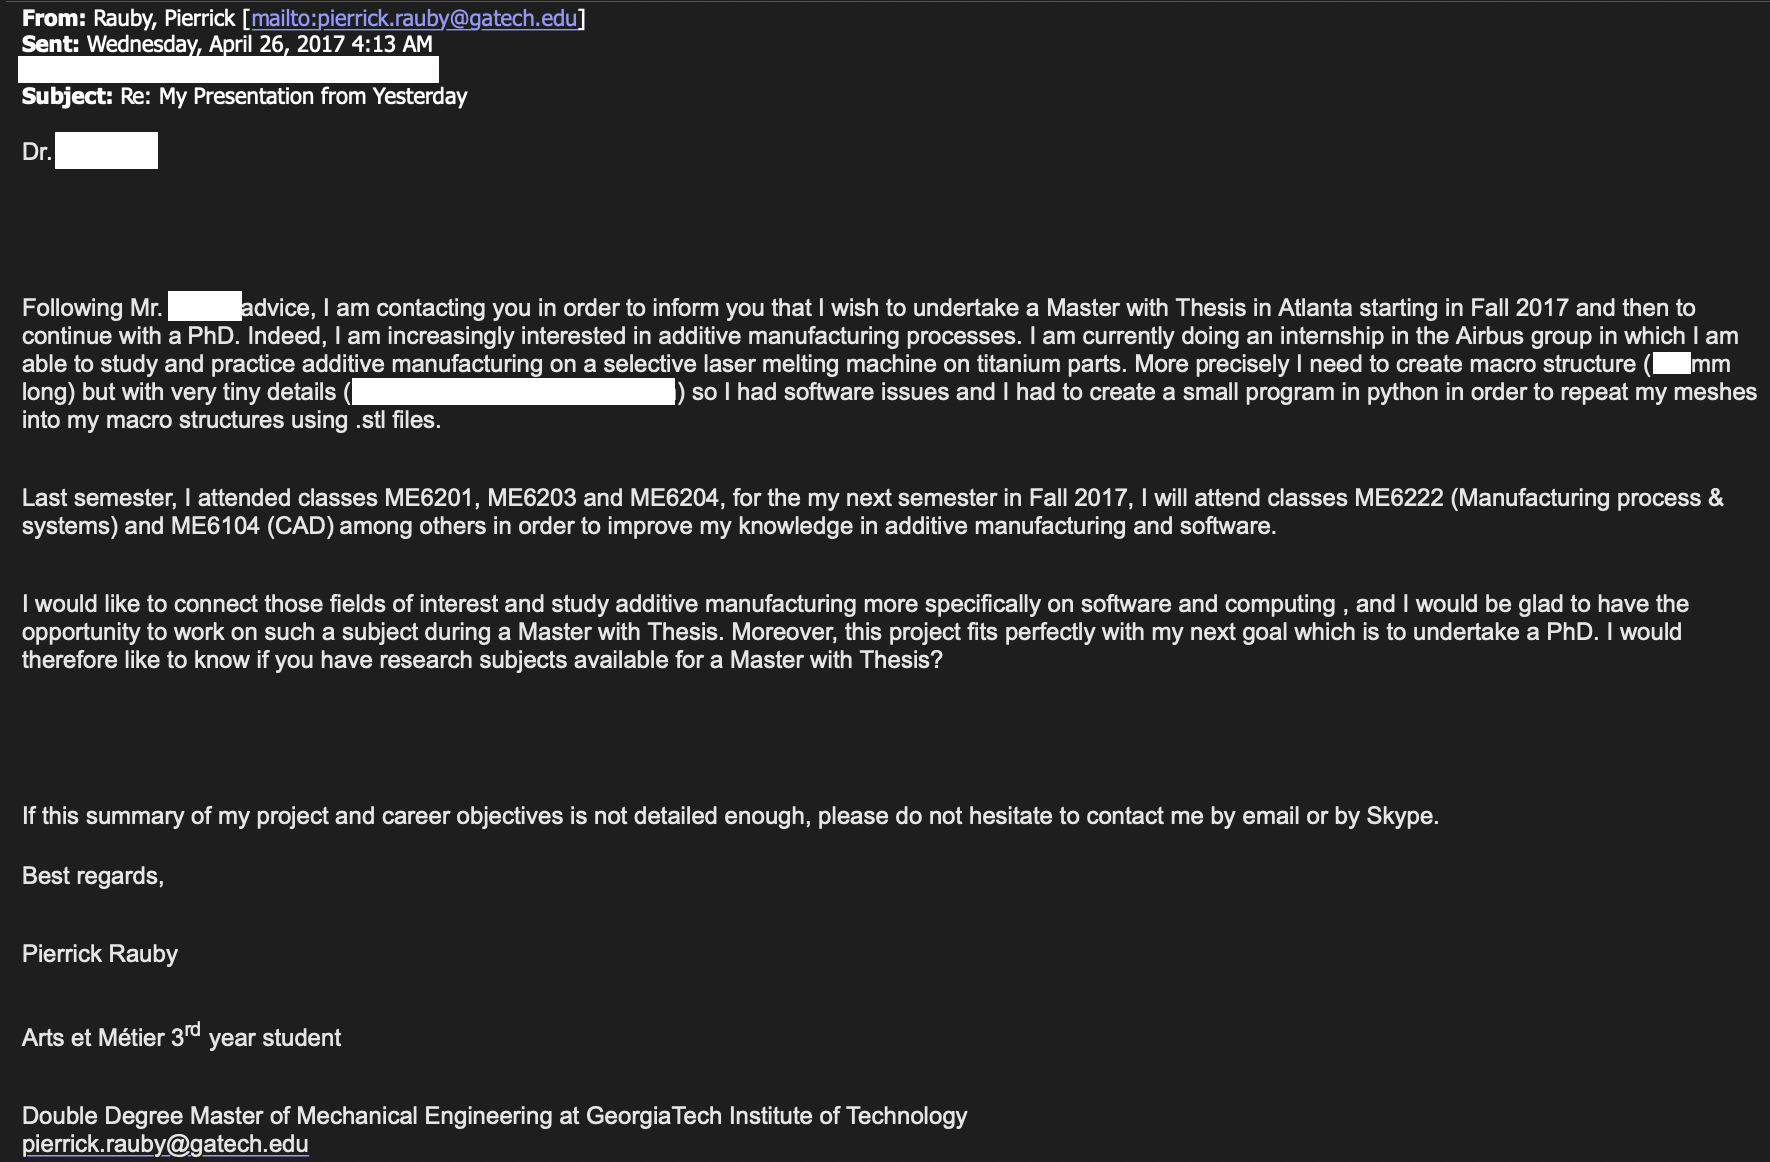
\includegraphics[width=14cm]{mail_Pierrick.png} 
\end{center}
\caption{Contact suite a un piston}
\label{Contact suite a un piston}
\end{figure}
\newpage
\subsection{Contact spécifique vers un prof}
\begin{figure}[h]
\begin{center}
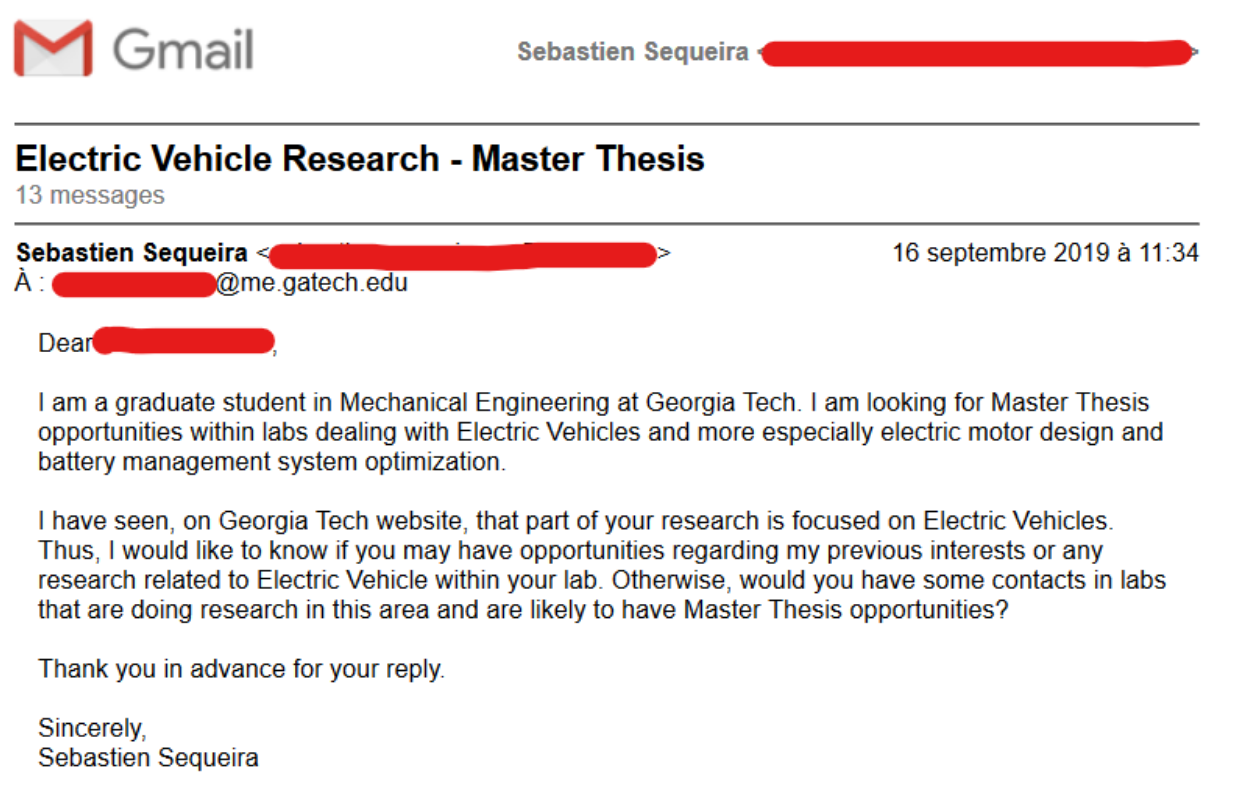
\includegraphics[width=14cm]{Electric_vehicle.png} 
\end{center}
\caption{Contact d'un prof specifique}
\label{Contact d'un prof specifique}
\end{figure}
\newpage

\subsection{Prise de contact un peu plus générale}
\begin{figure}[h]
\begin{center}
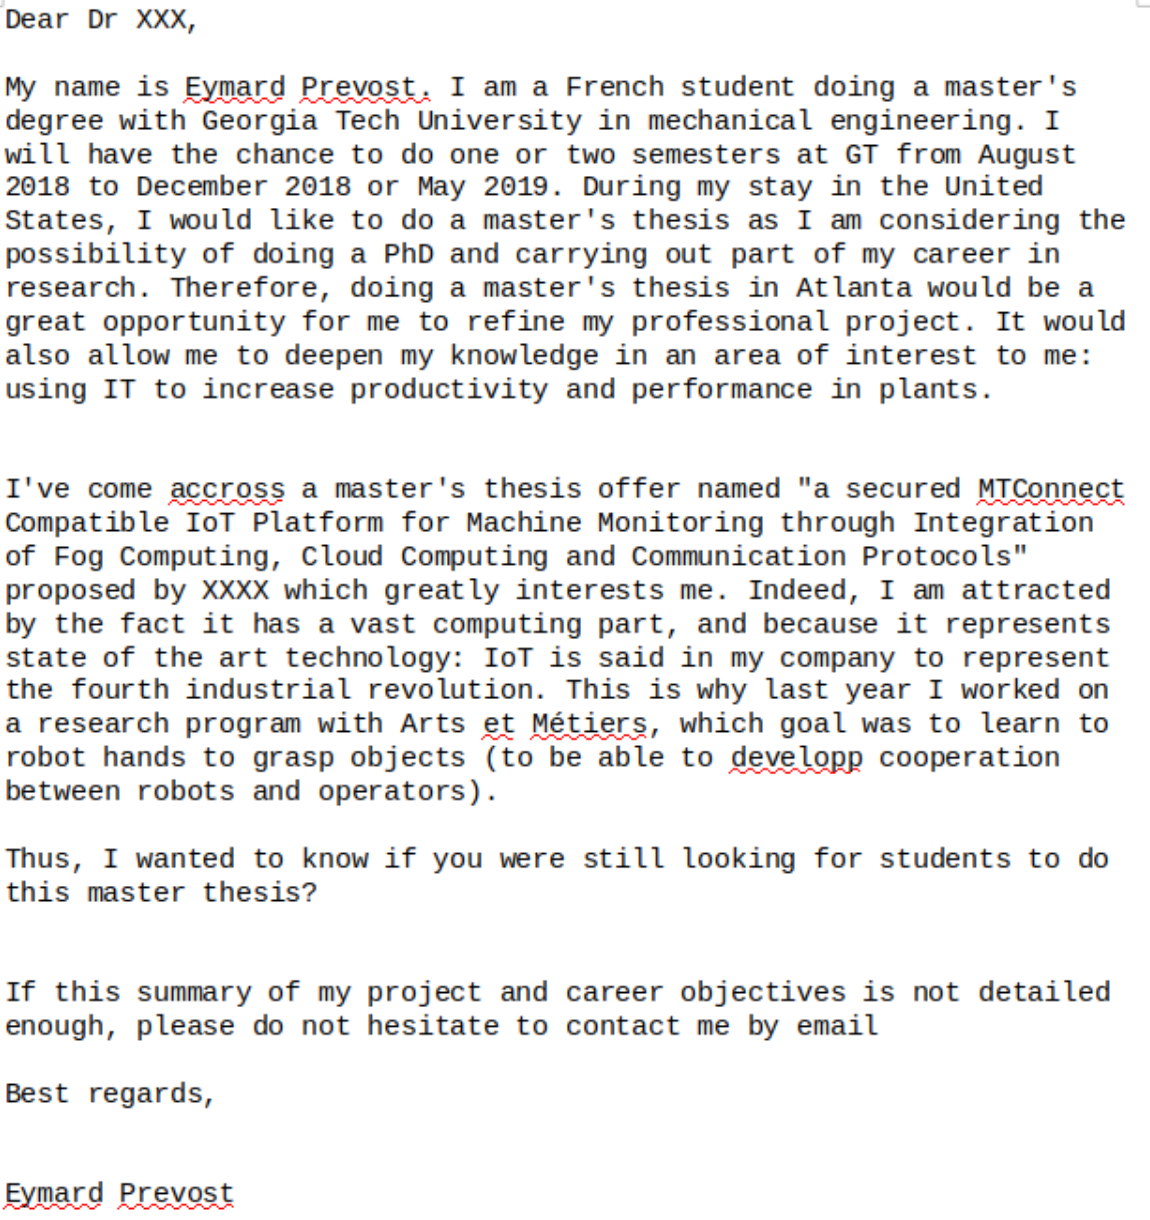
\includegraphics[width=14cm]{mail_Eymard.png} 
\end{center}
\caption{Contact plus general}
\label{Contact plus generale}
\end{figure}


\end{document}


